\documentclass{article}
\usepackage[utf8]{inputenc} % Indica cuál es la codificación de este archivo
\usepackage[spanish]{babel} % Indica el idioma en que está escrito el documento

\usepackage{listings}
\usepackage{xcolor}
\usepackage{graphicx}
% Define un estilo para el código C
\lstdefinestyle{mystyle}{
    backgroundcolor=\color{gray!10},
    basicstyle=\ttfamily,
    breakatwhitespace=false,
    breaklines=true,
    captionpos=b,
    commentstyle=\color{green!40!black},
    keywordstyle=\color{blue},
    numbers=left,
    numbersep=5pt,
    numberstyle=\tiny\color{gray},
    showspaces=false,
    showstringspaces=false,
    showtabs=false,
    tabsize=2
}
\begin{document}
\title{Lenguaje de programación C}
\maketitle
\section{Introducción}

El lenguaje fue concebido por Dennis Ritchie, le inventó en 1972. Su propósito era escribir un sistema operativo, el mismo que en contemporaneidad conocemos denominado como Unix. A veces se dice que C es un ensamblador portátil; es un sistema de implementación de sistemas. Depende, además de otros lenguajes, del diseño prístino de Algol 60. Algol 60 fue un lenguaje codificado por un grupo internacional de científicos de la computación en 1960, justo al principio de la existencia de ciencias de la computación; muchos de los conceptos que a día de hoy empleamos han nacido o comenzado con Algol 60. Es el resultado de dos lenguajes anteriores, el BCPL y el B. Fueron Kernighan y Ritchie los que publicaron una descripción definitiva del lenguaje conocida como "K\&R C". \\

\begin{quotation}
A raiz de la creciente popularidad de los microordenadores, comenzaron a surgir numerosas implementaciones de C que diferían en parte de la definición de K\&R, creando pequeñas incompatibilidades y disminuyendo la portabilidad del lenguaje. Esto hizo necesaria la búsqueda de un C estandard, representado por el ANSI C.*\\
\end{quotation}

Originalmente el Lenguaje C estuvo muy ligado al sistema operativo UNIX que, en su mayor parte, está escrito en C. Más adelante se comenzó a utilizar en otros sistemas operativos para programar editores, compiladores, etc. Aunque se le conoce como un lenguaje de programación de sistemas, no se adapta mal al resto de aplicaciones. De hecho, hoy en día un alto porcentaje de software para ordenadores personales está escrito en Lenguaje C. Por ejemplo, el sistema operativo MS-DOS.

\subsection{Estructura de un Programa en C}
Un programa en C se compone de funciones. La función principal es `main()`, y es el punto de entrada de un programa C.

\begin{lstlisting}[style=mystyle, language=C]
#include <stdio.h>
int main() {
    printf("Hello world");
    return 0;
}
\end{lstlisting}
\texttt{\#include \<stdio.h\>} es una directiva de preprocesador que le indica al compilador que incluya el archivo de encabezado (header) stdio.h. Este archivo es una biblioteca que contiene las declaraciones necesarias para usar funciones de entrada-salida estándar, como printf. \texttt{\#include} es una palabra especial que le dice al compilador que la siguiente librería debe ser incluida, en este preciso ejemplo ya hemos hecho uso de la "\texttt{standar IO (Input-Output)": \<stdio.h\>} \\

\begin{lstlisting}[style=mystyle, language=C]
int main() {
\end{lstlisting}
La línea \texttt{int main()} define la función principal del programa, llamada main. Es el punto de entrada de cualquier programa en C.\\

\begin{lstlisting}[style=mystyle, language=C]
return 0; 
\end{lstlisting}
La línea \texttt{return 0}; indica que el programa ha finalizado exitosamente y devuelve el valor 0 al sistema operativo. Este valor se utiliza a menudo para indicar que el programa se ejecutó correctamente. Sin embargo, el uso de return 0; en main es opcional en lenguaje C moderno, ya que se asume un valor de retorno de 0 si no se proporciona explícitamente.

\section{Por qué}
Existen variopintos aspectos, cada cual adecuado para la enseñanza principiante; no hay nada equivocado al empezar con un lenguaje u otro: sin embargo, aunque se conozca Python, Java o cualquier otro, apreciaremos el aprendizaje de C. Fue inventado por Bell Labs en 1972, y es un lenguaje empleado en toda clase de industria, es a lo que llamamos un lenguaje de implementación de sistemas. Aprender lenguajes tales como Java o Python, si bien no es en absoluto mal, se deberá tener de igual manera en consideración los detalles que ocultados subyacen a tales lenguajes para su mejor digestión, pero, en cuanto al avance, aprendizaje o comprensión de lo que un proceso computacional realiza, requeriremos un lenguaje que pueda dotarnos de un mayor acercamiento al sólido metal desnudo.

\section{Tipos de dato}
En la programación en C, los tipos de datos son declaraciones de variables. Esto determina el tipo y el tamaño de los datos asociados con las variables. Por ejemplo:

\begin{lstlisting}[style=mystyle, language=C]
char a = 'C'; // single character    %c
char b[] = "Bro"; // array of characters %s  

float c = 3.141592; // 4 bytes (32 bits of precision) 6 - 7 digits %f
double d = 3.141592653589793; // 8 bytes (64 bits of precision) 15 - 16 digits %lf

bool e = true; // 1 byte (true or false) %d

char f = 120; // 1 byte (-128 to +127) %d or %c
unsigned char g = 255; // 1 byte (0 to +255) %d or %c

short h = 32767; // 2 bytes (−32,768 to +32,767) %d
unsigned short i = 65535;  // 2 bytes (0 to +65,535) %d

int j = 2147483647; // 4 bytes (-2,147,483,648 to +2,147,483,647) %d
unsigned int k = 4294967295;  // 4 bytes (0 to +4,294,967,295) %u

long long int l = 9223372036854775807; // 8 bytes (-9 quintillion to +9 quintillion) %lld
unsigned long long int m = 18446744073709551615U; // 8 bytes (0 to +18 quintillion) %llu

printf("%c\n", a);  // char
printf("%s\n", b);  // character array
printf("%f\n", c);  // float
printf("%lf\n", d); // double
printf("%d\n", e);  // bool
printf("%d\n", f);  // char as numeric value
printf("%d\n", g);  // unsigned char as numeric value
printf("%d\n", h);  // short
printf("%d\n", i);  // unsigned short
printf("%d\n", j);  // int
printf("%u\n", k);  // unsigned int
printf("%lld\n", l);  // long long int
printf("%llu\n", m);  // unsigned long long int
\end{lstlisting}
\subsection{Int}
Aquí, es una variable de tipo (entero). Los enteros son números enteros que pueden tener valores cero, positivos o negativos, pero no valores decimales. El tamaño de suele ser de 4 bytes (32 bits).

\begin{lstlisting}[style=mystyle, language=C]
// C program to print Integer data types.
#include <stdio.h>

int main()
{
	// Integer value with positive data.
	int a = 9;

	// integer value with negative data.
	int b = -9;

	// U or u is Used for Unsigned int in C.
	int c = 89U;

	// L or l is used for long int in C.
	long int d = 99998L;

	printf("Integer value with positive data: %d\n", a);
	printf("Integer value with negative data: %d\n", b);
	printf("Integer value with an unsigned int data: %u\n",
		c);
	printf("Integer value with an long int data: %ld", d);

	return 0;
}
\end{lstlisting}

\subsection{Float}
En la programación C, el [tipo de datos] punto-flotante se utiliza para almacenar valores de coma flotante. Float en C se utiliza para almacenar valores decimales y exponenciales. Se utiliza para almacenar números decimales (números con valores de coma flotante) con precisión simple.

\begin{lstlisting}[style=mystyle, language=C]
// C Program to demonstrate use
// of Floating types
#include <stdio.h>

int main()
{
	float a = 9.0f;
	float b = 2.5f;

	// 2x10^-4
	float c = 2E-4f;
	printf("%f\n", a);
	printf("%f\n", b);
	printf("%f", c);

	return 0;
}
\end{lstlisting}

\subsection{Void}
El tipo de datos void en C se utiliza para especificar que no hay ningún valor presente. No proporciona un valor de resultado a su autor de la llamada. No tiene valores ni operaciones. Se utiliza para no representar nada. Void se usa de varias maneras como tipo de retorno de función, argumentos de función como void y [punteros a void].

\begin{lstlisting}[style=mystyle, language=C]
// C program to demonstrate
// use of void pointers
#include <stdio.h>

int main()
{
	int val = 30;
	void* ptr = &val;
	printf("%d", *(int*)ptr);
	return 0;
}
\end{lstlisting}
\subsection{Tamaño de los tipo de datos}
El tamaño de los tipos de datos en C depende del tamaño de la arquitectura, por lo que no podemos definir el tamaño universal de los tipos de datos. Para eso, el lenguaje C proporciona el operador sizeof() para verificar el tamaño de los tipos de datos.

\begin{lstlisting}[style=mystyle, language=C]
// C Program to print size of
// different data type in C
#include <stdio.h>

int main()
{
	int size_of_int = sizeof(int);
	int size_of_char = sizeof(char);
	int size_of_float = sizeof(float);
	int size_of_double = sizeof(double);

	printf("The size of int data type : %d\n", size_of_int);
	printf("The size of char data type : %d\n",
		size_of_char);
	printf("The size of float data type : %d\n",
		size_of_float);
	printf("The size of double data type : %d",
		size_of_double);

	return 0;
}
\end{lstlisting}
\section{Especificadores de formato}
El especificador de formato en C se utiliza para informar al compilador sobre el tipo de datos que se imprimirán o escanearán en las operaciones de entrada y salida. Siempre comienzan con un símbolo \% y se utilizan en la cadena formateada en funciones como printf(), scanf, sprintf(), etc. El lenguaje C proporciona una serie de especificadores de formato que están asociados con los diferentes tipos de datos.
\begin{lstlisting}[style=mystyle, language=C]
#include <stdio.h>
int main(){
	// format specifier % = defines and formats a type of data to be displayed
	// %c = character
	// %s = string (array of characters)
	// %f = float
	// %lf = double
	// %d = integer
	// %.1 = decimal precision
	// %1 = minimum field width
	// %- = left align
	float item1 = 5.75;
	float item2 = 10.00;
	float item3 = 100.99;
	
	printf("Item 1: $%8.2f\n", item1);
	printf("Item 2: $%8.2f\n", item2);
	printf("Item 3: $%8.2f\n", item3);
	return 0;
}
\end{lstlisting}

\section{Operadores}
Los operadores son símbolos que indican cómo se deben manipular los operandos. Los operadores junto con los operandos forman una expresión, que es una fórmula que define el cálculo de un valor. Los operandos pueden ser constantes, variables o llamadas a funciones, siempre que éstas devuelvan algún valor. El compilador evalúa los operadores, algunos de izquierda a derecha, otros de derecha a izquierda, siguiendo un orden de precedencia. Este orden se puede alterar utilizando paréntesis para forzar al compilador a evaluar primero las partes que se deseen. Operadores. (ugr.es)

\begin{lstlisting}[style=mystyle, language=C]
#include <stdio.h>
int main(){
	// arithmetic operators
	// + (addition)
	// - (subtraction)
	// * (multiplication)
	// / (division)
	// % (modulus)
	// ++ increment
	// -- decrement
	
	int x = 5;
	int y = 2;
	
	// int z = x + y;
	// int z = x - y;
	// int z = x * y;
	// float z = x / (float) y;
	// int z = x % y;
	// x++;
	// y--;
	
	printf("%d", x);
	printf("%d", y);
	return 0;
}
\end{lstlisting}
\section{Variables}
Una variable es un elemento de datos con nombre cuyo valor puede cambiar durante el curso de la ejecución de un programa. Se les asigna espacio en la memoria para almacenar un valor al que nos referimos como nombre de la variable para acceder al dato o valor almacenado. La variable pasa a comportarse como si fuese el valor o dato que ella misma contiene en referencia al contenedor donde se encuentra susodicho valor. Para crear una variable, primero tenemos que declarar un nombre de la variable, precediéndole con el tipo de dato que estamos almacenando. La variable es creada en declaración e inicialización, dos pasos a realizar de manera respectiva, es decir, primero debemos declarar para asignar algo de espacio en la memoria por el cual se pueda almacenar el valor, e inicializar posteriormente.

\begin{lstlisting}[style=mystyle, language=C]
#include <stdio.h>
int main(){
	/* variable = Allocated space in memory to store a value.
				We refer to a variable's name to access the stored value.
				That variable now behaves as if it was the value it contains.
				BUT we need to declare what type of data we are storing.
	*/
	int x; // declaration = we are creating space in memory to store a value
	x = 123; //initialization
	int y = 321: // declaration + initialization
	return 0;
}
\end{lstlisting}

\section{Funciones}
Una función en C es un conjunto de sentencias que cuando se llaman realizan alguna tarea específica. Es el bloque de construcción básico de un programa C que proporciona modularidad o reutilización de código. Las sentencias de programación de una función están encerradas dentro de { } llaves, teniendo ciertos significados y realizando ciertas operaciones. También se les llama subrutinas o procedimientos en otros lenguajes.

\subsection{Declaraciones de una función}
En una declaración de función, debemos proporcionar el nombre de la función, su tipo de retorno y el número y tipo de sus parámetros. Una declaración de función le dice al compilador que hay una función con el nombre dado definido en otro lugar del programa.

\subsubsection{Sintaxis}
\texttt{return\_type \*\*name\_of\_the\_function\*\* (\_parameter\_1\_, \_parameter\_2\_);} \\
El nombre del parámetro no es obligatorio al declarar funciones. También podemos declarar la función sin usar el nombre de las variables de datos. Ejemplo: 
\texttt{int \*\*sum\*\*(int \_a\_, int \_b\_);\\
int \*\*sum\*\*(int , int);} \\

\subsubsection{Definición de funciones}
La definición de la función consiste en sentencias reales que se ejecutan cuando se llama a la función (es decir, cuando el control del programa llega a la función). Una función C generalmente se define y declara en un solo paso porque la definición de la función siempre comienza con la declaración de función, por lo que no necesitamos declararla explícitamente. El ejemplo siguiente sirve como definición de función y como declaración.\\

\texttt{return\_type \*\*function\_name\*\* (para1\_type \_para1\_name,\_ para2\_type \_para2\_name\_) \\
\{
   \_//body of the function\_
\}
}
\subsubsection{Llamada de una función}
Una llamada a función es una instrucción que indica al compilador que ejecute la función. Usamos el nombre de la función y los parámetros en la llamada a la función. En el ejemplo siguiente, se llama a la primera función de suma y 10,30 se pasa a la función de suma. Después de la función, la suma de llamada de a y b se devuelve y el control también se devuelve a la función principal del programa.
\begin{figure}[h]
    \centering
    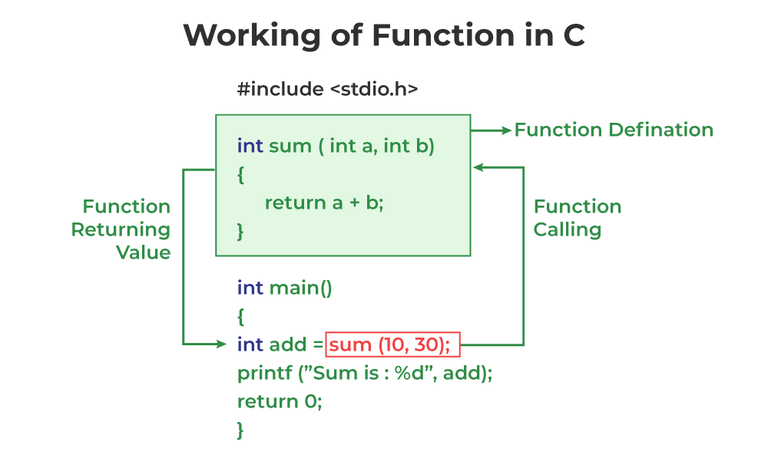
\includegraphics[width=1\linewidth]{254468247-faf2807d-14dc-45dc-9d7c-c137fc717a89.png}
    \caption{Enter Caption}
    \label{fig:enter-label}
\end{figure}
\section{Tipos de funciones}
Hay dos tipos de funciones en C:
\begin{itemize}
    \item Funciones de la biblioteca
    \item Funciones definidas por el usuario
\end{itemize}
\begin{figure}[h]
    \centering
    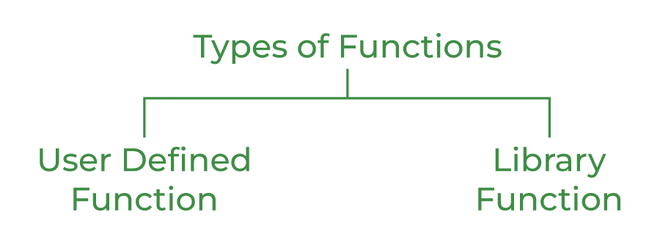
\includegraphics[width=1\linewidth]{254468287-72e1c799-37f9-40ed-b781-809832e3ba5b.png}
    \caption{Enter Caption}
    \label{fig:enter-label}
\end{figure}
\subsubsection{Función de biblioteca}
Una función de [biblioteca] también se conoce como una "función incorporada". Ya existe un paquete compilador que contiene estas funciones, cada una de las cuales tiene un significado específico y se incluye en el paquete. Las funciones integradas tienen la ventaja de ser directamente utilizables sin ser definidas, mientras que las funciones definidas por el usuario deben declararse y definirse antes de ser utilizadas. \\

\texttt{pow(), sqrt(), strcmp(), strcpy() etc.} \\

Están optimizadas para un mejor rendimiento, y ahorran mucho tiempo, es decir, tiempo de desarrollo de funciones. Ej.
\begin{lstlisting}[style=mystyle, language=C]
// C program to implement
// the above approach
#include <math.h>
#include <stdio.h>

// Driver code
int main()
{
double Number;
Number = 49;

// Computing the square root with
// the help of predefined C
// library function
double squareRoot = sqrt(Number);

printf("The Square root of %.2lf = %.2lf",
		Number, squareRoot);
return 0;
}
\end{lstlisting}
\subsubsection{Funciones definidas}
Las funciones que crea el programador se conocen como funciones definidas por el usuario o "funciones a medida". Las funciones definidas por el usuario se pueden mejorar y modificar según las necesidades del programador. Cada vez que escribimos una función que es específica de mayúsculas y minúsculas y no está definida en ningún archivo de cabecera, necesitamos declarar y definir nuestras propias funciones de acuerdo con la sintaxis.

\begin{lstlisting}[style=mystyle, language=C]
#include <stdio.h>
void functionName()
{
    ... .. ...
    ... .. ...
}

int main()
{
    ... .. ...
    ... .. ...

    functionName();
    
    ... .. ...
    ... .. ...
}
\end{lstlisting}
La ejecución de un programa C comienza desde la función \texttt{main()} Cuando el compilador encuentra el control del programa salta a \texttt{functionName();}

\section{Parametros a funciones}
Los datos pasados cuando se invoca la función se conocen como parámetros reales. En el siguiente programa, 10 y 30 se conocen como parámetros reales. Los parámetros formales son la variable y el tipo de datos mencionados en la declaración de funciones. En el siguiente programa, a y b se conocen como parámetros formales.

\begin{figure}[h]
    \centering
    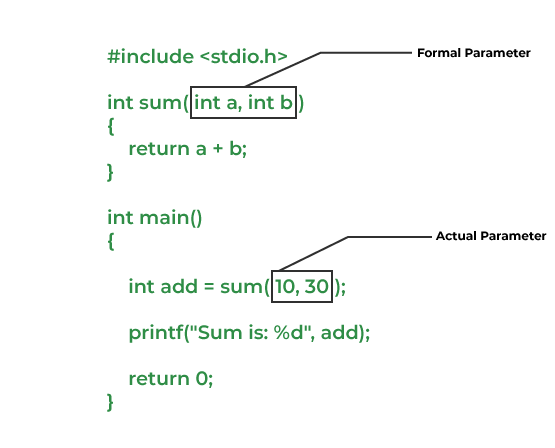
\includegraphics[width=1\linewidth]{254468322-f11bd144-af1f-49b8-a371-06aa739e38e0.png}
    \caption{Enter Caption}
    \label{fig:enter-label}
\end{figure}
\begin{lstlisting}[style=mystyle, language=C]
#include <stdio.h>
void birthday()
{
   printf("\nHappy birthday to you!");
   printf("\nHappy birthday to you!");
   printf("\nHappy birthday dear...YOU!");
   printf("\nHappy birthday to you!\n");
}
int main()
{
   birthday();
   birthday();
   birthday();
   return 0;
}
\end{lstlisting}
Se puede llamar a una función varias veces para proporcionar reutilización o modularidad. Mediante el uso de funciones, podemos evitar reescribir la misma lógica / código una y otra vez en un programa; la reutilización es el principal logro de las funciones C.
\section{Parametros}
Se puede llamar a una función varias veces para proporcionar reutilización o modularidad. Mediante el uso de funciones, podemos evitar reescribir la misma lógica / código una y otra vez en un programa; la reutilización es el principal logro de las funciones C.

\begin{lstlisting}[style=mystyle, language=C]
void sumar(int a, int b) {  // a y b son parametros, básicamente
			   // definiciones de las variables que almacenarán
			  // los valores correspondientes al argumento
    int resultado = a + b;
    printf("La suma es: %d\n", resultado);
}
\end{lstlisting}
\section{Argumentos}
Los argumentos son los valores reales que se pasan a una función cuando es llamada. Estos valores deben coincidir en tipo y número con los parámetros definidos en la función. Cuando se llama a una función, se proporcionan los argumentos que corresponden a los parámetros de la función. Estos argumentos son los valores que se utilizarán en la ejecución de la función.
\begin{lstlisting}[style=mystyle, language=C]
int main() {
    int x = 5;
    int y = 10;
    sumar(x, y);  // Aquí x e y son los argumentos que se pasan a la función
		 // sumar, estos son los valores que se almacenarán en las
		// variables declaradas como parametro.
    return 0;
}
\end{lstlisting}
Cuando definimos una función, se especifican los parámetros requeridos, y se le asginan nombres / denominaciones. Estos parámetros se comportan como variables locales dentro de la función y se utilizan para recibir valores que se pasarán a la función cuando sea llamada. Los argumentos son los valores reales que se pasan a la función cuando es llamada. Estos valores deben coincidir en tipo y número con los parámetros definidos en la función. Cuando llamamos a una función, proporcionamos los argumentos que se almacenarán en los parámetros de la función. Estos argumentos son los valores que la función utilizará en su ejecución. En resumen:\\
\begin{itemize}
    \item Los parámetros son las variables definidas en la declaración de la función.
    \item Los argumentos son los valores reales pasados a la función, y que se almacenarán en los parámetros
\end{itemize}
\section{Operadores lógicos}
Los operadores lógicos en C se utilizan para combinar múltiples condiciones/restricciones. Operadores lógicos devuelve 0 o 1, depende del resultado de la expresión true o false. En la programación C para la toma de decisiones, utilizamos operadores lógicos. Tenemos 3 operadores lógicos principales en el lenguaje:
\begin{itemize}
    \item \texttt{Lógico Y (\&\&)}
    \item \texttt{Lógico O (||)}
    \item \texttt{Lógico NO (!)}
    \item \texttt{XOR lógico(\^)}
\end{itemize}
\subsection{Tipos de operadores lógicos}
\subsubsection{Operador lógico AND}
Si ambos operandos son distintos de cero, entonces la condición se convierte en verdadera. De lo contrario, el resultado tiene un valor de 0. El tipo de retorno del resultado es int. A continuación se muestra la tabla de verdad para el operador lógico AND.\\

\begin{tabular}{|c|c|c|}
\hline
X & Y & X \&\& Y \\
\hline
1 & 1 & 1 \\
1 & 0 & 0 \\
0 & 1 & 0 \\
0 & 0 & 0 \\
\hline
\end{tabular}

\subsection{Operador lógico OR}
La condición se convierte en verdadera si cualquiera de ellos es distinto de cero. De lo contrario, devuelve false, es decir, 0 como valor. A continuación se muestra la tabla de verdad para el operador OR lógico.\\

\begin{tabular}{|c|c|c|}
\hline
X & Y & X|Y \\
\hline
1 & 1 & 1 \\
1 & 0 & 1 \\
0 & 1 & 1 \\
0 & 0 & 0 \\
\hline
\end{tabular}

\subsection{Operador lógico NOT}
Si la condición es verdadera, entonces el operador lógico NOT la hará falsa y viceversa. A continuación se muestra la tabla de verdad para el operador NOT. \\

\begin{tabular}{|c|c|}
\hline
X & !X \\
\hline
0 & 1 \\
1 & 0 \\
\hline
\end{tabular}

\subsection{Operador lógico XOR}
Si ambos bits son iguales, devolverá false de lo contrario true. A continuación se muestra la tabla de verdad para el operador XOR lógico.\\

\begin{tabular}{|c|c|c|}
\hline
X & Y & X$^Y$ \\
\hline
0 & 0 & 0 \\
0 & 1 & 1 \\
1 & 0 & 1 \\
1 & 1 & 0 \\
\hline
\end{tabular}
\subsection{Práctica}
\begin{lstlisting}[style=mystyle, language=C]
// C program to demonstrate
// Logical Operators
#include <stdio.h>

// Driver code
int main()
{
int x = 7, y = 3;

// Logical operators
printf("Following are the logical operators in C \n");
printf("The value of this logical and operator ((x==y) "
		"&& (x<y)) is: %d \n",
		((x == y) && (x < y)));

printf("The value of this logical or operator ((x==y) "
		"|| (x<y)) is: %d \n",
		((x == y) || (x < y)));

printf("The value of this logical not operator "
		"(!(x==y)) is: %d ",
		(!(x == y)));
return 0;
}
\end{lstlisting}

\section{Evaluación de cortocircuito}
El cortocircuito es uno de los pasos de optimización del compilador, en este paso se evita el cálculo innecesario durante la evaluación de una expresión. La expresión se evalúa de izquierda a derecha. Funciona en ciertos casos en los que el valor de la expresión se puede calcular ciertamente evaluando solo partes de la expresión.\\

Evaluación de cortocircuito: el [compilador] omite la ejecución o evaluación de algunas subexpresiones en una expresión lógica. El compilador deja de evaluar las subexpresiones adicionales tan pronto como se determina el valor de la expresión. A continuación se muestra un ejemplo de lo mismo:
\begin{lstlisting}[style=mystyle, language=C]
if (a == b || c == d || e == f) {
	// do_something
}
\end{lstlisting}
Si la expresión \texttt{a == b} es verdadera, entonces \texttt{c == d} y \texttt{e == f} no se evalúan porque el resultado de la expresión ya ha sido determinado. Del mismo modo, si se usamos el \texttt{[operador lógico AND (\&\&] en lugar de OR lógico (||)}, y la expresión \texttt{a == b} es false, el compilador omitirá evaluar otras subexpresiones.
\begin{lstlisting}[style=mystyle, language=C]
#include <stdio.h>
int main(){
	int outside, weather;
	printf("\nIf outside 1 true 0 false:");
	scanf("%d", &outside);
	printf("\nIf rain 1 true 0 false:");
	scanf("%d", &weather);
	if (outside && weather) {
	printf("\nUse an umbrella");
	}
	else {
	printf("\nDress normally");
	}
	return 0;
}
\end{lstlisting}
\end{document}